\documentclass[12pt]{article}
\usepackage[T2A]{fontenc}
\usepackage[utf8]{inputenc}
\usepackage[russian]{babel}
\usepackage{amsmath, graphicx, float, hyperref, pgf, cite}

\DeclareMathOperator{\sign}{sign}
\DeclareMathOperator{\MyIm}{Im}

\graphicspath{{./pictures/}}

\hypersetup{
    colorlinks=true,
    linkcolor=blue,
    urlcolor=cyan,
    citecolor=magenta,
}

\begin{document}
    \begin{titlepage}
        \begin{center}
            \vspace*{1cm}

            \Huge
            \textbf{Закон всемирного тяготения.\\Точки Лагранжа}

            \vspace{1.5cm}

            \Large
            \textbf{Балдин Виктор Б01-303}

            \vfill

            Вопрос по выбору \\
            Устный экзамен по общей физике

            \vspace{0.8cm}

            
\includegraphics[width=0.4\textwidth]{university_logo.png}

            Физтех-школа радиотехники и компьютерных технологий\\
            Московский физико-технический институт\\
            Долгопрудный, 2024
        \end{center}
    \end{titlepage}

    \begin{abstract}
        \par Данный вопрос по выбору включает в себя теоретические расчеты
        положения точек Лагранжа и обсуждение некоторых их интересных
        свойств. В работе используются материалы из различных открытых
        источников об истории исследований на эту тему и современном их
        состоянии.
        \par Точки Лагранжа являются крайне важным объектом для изучения
        космического пространства в современной астрофизике.
        В частности, прямым образом их свойства используются для размещения
        космических аппаратов, предназначенных для наблюдений дальнего
        космоса.
        \par Автор выражает надежду, что данная работа содержит
        актуальные сведения и благодарит экзаменационную комиссию за ее
        рассмотрение.
    \end{abstract}

    \newpage

    \section{Введение}
    \par \textit{Точки Лагранжа}, в некоторых источниках также \textit{точки
    либрации} или \textit{$L$-точки} -- точки в системе двух тел, в которых
    третье тело может оставаться неподвижным относительно первых двух.
    \par Точки Лагранжа названы в честь математика Жозефа Луи Лагранжа,
    который первым в 1772 году показал их существование.

    \begin{figure}[H]
        \centering
        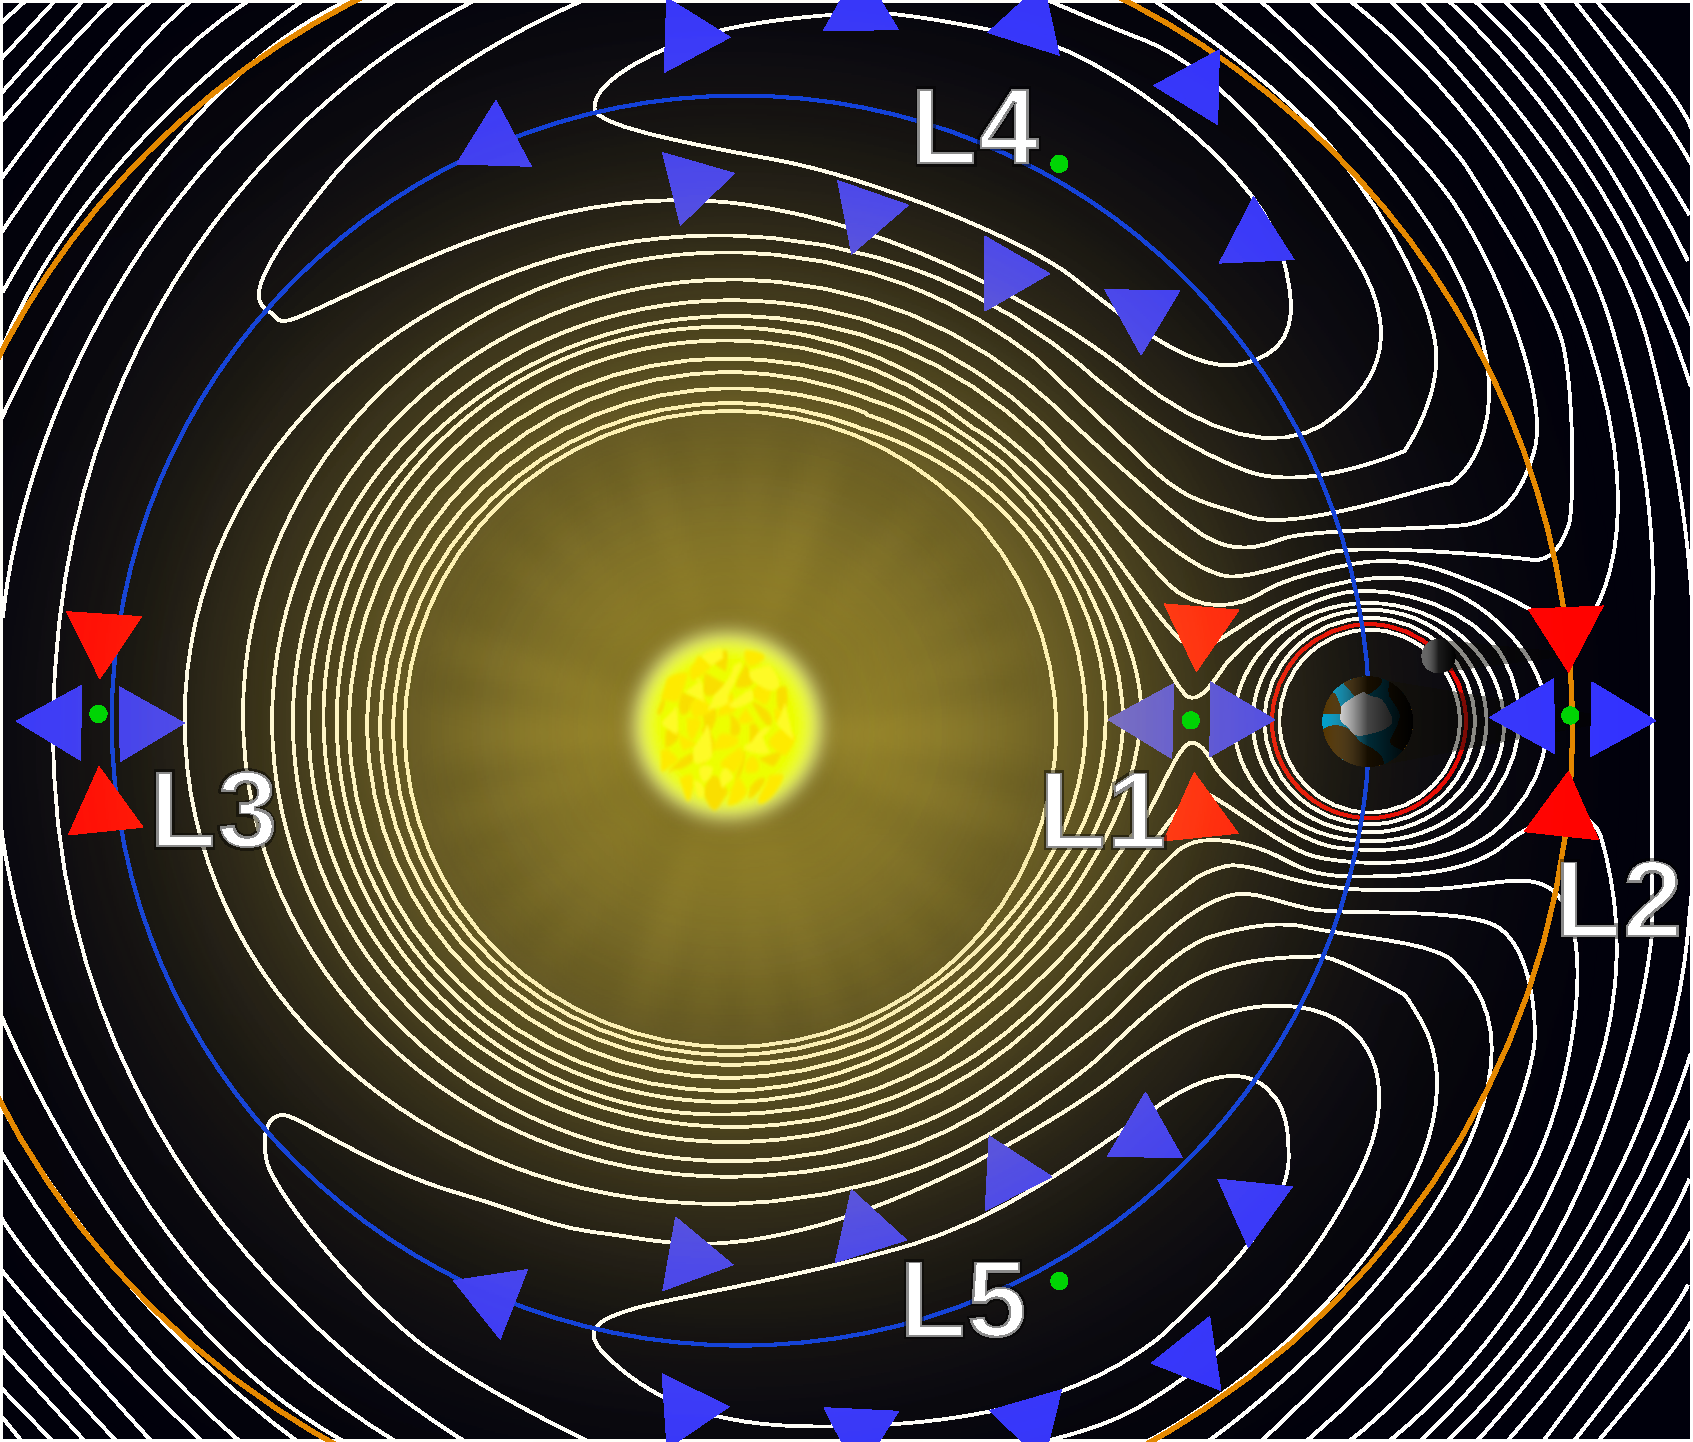
\includegraphics[scale=0.35]{Lagrange_points.pdf}
        \caption{5 точек Лагранжа и гравитационные эквипотенциальные
        поверхности системы двух тел\\
        \textit{Источник:}
        \url{https://upload.wikimedia.org/wikipedia/commons/thumb/e/ee/
        Lagrange_points2.svg/1920px-Lagrange_points2.svg.png}}
        \label{points}
    \end{figure}

    \section{Точки Лагранжа}
    \par Для начала проведем краткое рассмотрение движения 3-х тел, связанных между
    собой гравитационными взаимодействиями. Это может быть описано в общем
    случае следующими дифференциальными уравнениями \cite{mit2008}:

    \begin{equation}
        \begin{cases}
            \ddot{\vec{r_1}} = -Gm_2\frac{\vec{r_1} - \vec{r_2}}
            {\lvert \vec{r_1} - \vec{r_2} \rvert} -
            Gm_3\frac{\vec{r_1} - \vec{r_3}}{\lvert \vec{r_1} - 
            \vec{r_3} \rvert}\\
            \ddot{\vec{r_2}} = -Gm_2\frac{\vec{r_2} - \vec{r_3}}
            {\lvert \vec{r_2} - \vec{r_3} \rvert} -
            Gm_3\frac{\vec{r_2} - \vec{r_1}}{\lvert \vec{r_2} - 
            \vec{r_1} \rvert}\\
            \ddot{\vec{r_3}} = -Gm_2\frac{\vec{r_3} - \vec{r_1}}
            {\lvert \vec{r_3} - \vec{r_1} \rvert} -
            Gm_3\frac{\vec{r_3} - \vec{r_2}}{\lvert \vec{r_3} - 
            \vec{r_2} \rvert}\\
        \end{cases}\,.
    \end{equation}

    Данная система имеет множество сложных решений, на которых мы не будем
    останавливаться. В нашу задачу входит частный случай задачи трех тел 
    (англ. \textit{restricted three-body problem}), в котором имеем
    2 массивных тела массами $M_1$ и $M_2$ и третье тело массой $m$, 
    $m \ll M_1$, $m \ll M_2$. В таком случае мы можем рассматривать движение
    $M_1$ и $M_2$ в рамках задачи двух тел, пренебрегая гравитационным
    воздействием третьего тела.
    \par Как известно, два тела в отсутствии внешних гравитационных воздейстсвий
    вращаются относительно центра масс системы. Мы будем рассматривать случай,
    когда они вращаются по окружности. Поэтому теперь мы можем
    поставить задачу конкретнее: найти все возможные положения третьего тела,
    при которых оно будет совершать вращение вокруг центра масс с той же угловой
    скоростью, что и $M_1$ и $M_2$. Логично ввести систему координат с началом в
    центре масс системы. Обозначим радиус-векторы $M_1$ и $M_2$ через $\vec{r_1}$
    и $\vec{r_2}$ соответственно.

    \begin{figure}[H]
        \centering
        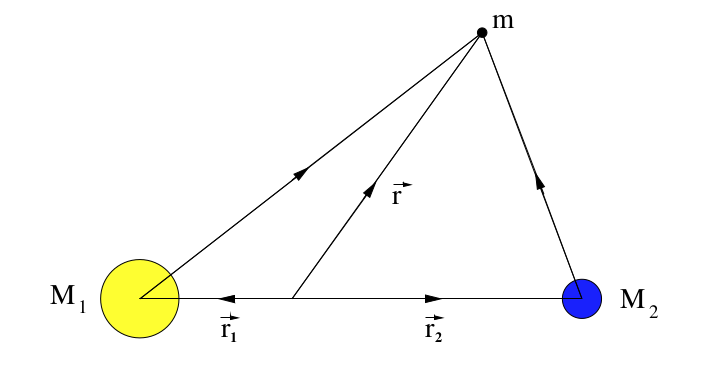
\includegraphics[scale = 2]{two-bodies.png}
        \caption{Рассматриваемый частный случай задачи трех тел \cite{nasagov}}
    \end{figure}

    Понятно, что теперь мы можем написать уравнение для ускорения тела $m$, 
    исходя из второго закона Ньютона и закона всемирного тяготения:
    
    \begin{equation}
        \vec{a} = \ddot{\vec{r}} = -\frac{GM_1}{\lvert \vec{r} - \vec{r_1} \rvert^3}
        (\vec{r} - \vec{r_1}) - \frac{GM_2}{\lvert \vec{r} - \vec{r_2} \rvert^3}
        (\vec{r} - \vec{r_2}) 
        \label{acceleration}
    \end{equation}

    \par Теперь из третьего закона Кеплера \cite{sivykhin} найдем угловую 
    скорость вращения системы $M_1$ и $M_2$:

    \begin{equation}
        \Omega^2 R^3 = G(M_1 + M_2), 
        \label{kepler}
    \end{equation}

    где $R$ -- расстояние между телами. Здесь используется, что $M_1$ и $M_2$ вращаются
    по окружностям радиусов $r_1$ и $r_2$ соответственно.

    \par Введем обозначения:
    \begin{equation}
        \alpha = \frac{M_2}{M_1 + M_2},\\\ \beta = \frac{M_1}{M_1 + M_2}
        \label{alpha_delta}
    \end{equation}

    \par Для дальнейших рассуждений полезно ввести ортонормированный
    базис: $\vec{k} = \frac{\vec{\Omega}}{\lvert \vec{\Omega} \rvert}$, 
    $\vec{i} = \frac{\vec{r_2}}{\lvert \vec{r_2} \rvert}$, $\vec{j} =
    [ \vec{k}, \vec{i} ]$. В этом базисе:

    % TODO: picture.
    \begin{eqnarray*}
        \vec{r}   = x(t)\vec{i} + y(t)\vec{j}\\
        \vec{r_1} = -\alpha R\vec{i}\\
        \vec{r_2} = \beta R\vec{i}
    \end{eqnarray*}

    Теперь напишем ускорение тела в системе отсчета, свзянной с $M_1$ и $M_2$.
    
    \begin{equation}
        \vec{a}_{\Omega} = \vec{a} - 2[\vec{\Omega}, \dot{\vec{r}}] - 
                            [\vec{\Omega}, [\vec{\Omega}, \vec{r}]]
        \label{a_omega}
    \end{equation}

    Так как мы ищем решения, для которых $\dot{\vec{r}} = 0$, это
    позволяет нам избавиться от ускорения Кориолиса. Таким образом, подставив 
    $\vec{a}$ из \ref{acceleration} в формулу \ref{a_omega} и заменив
    комбинации вида $GM$ через \ref{kepler}, получим:

    \begin{equation}
        \vec{a}_{\Omega} = \Omega^2
        \begin{pmatrix}
            x - \frac{\beta (x + \alpha R)R^3}{((x + \alpha R)^2 + y^2)^{3/2}} - 
            \frac{\alpha (x - \beta R)R^3}{((x - \beta R)^2 + y^2)^{3/2}} \\
            y - \frac{\beta y R^3}{((x + \alpha R)^2 + y^2)^{3/2}} - 
            \frac{\alpha y R^3}{((x - \beta R)^2 + y^2)^{3/2}}
        \end{pmatrix}
    \end{equation}

    \par Так как точки Лагранжа являются точками, в которых тело $m$ может пребывать в 
    состоянии равновесия в данной вращающейся системе отсчета, все возможные решения
    $(x,y)$ поставленной задачи можно найти из уравнения $\vec{a}_{\Omega} = 0$.

    \par Получаем систему из двух уравнений. Несложно заметить, что равненство
    нулю компоненты по оси $y$ ветвится на 2 случая. Для начала рассмотрим 
    случай $y = 0$. Чтобы немного упростить уравнение, 
    целесообразно сделать замену $x = R(u + \beta)$. В самом деле, так как
    из \ref{alpha_delta} $\alpha + \beta = 1$, получаем $x + \alpha R = (u + 1)R$,
    $x - \beta R = uR$. 
    
    \par Теперь подставим $y$ в первое уравнение системы. Для краткости
    введем обозначения $s_0 = \sign(u)$, $s_1 = \sign(u + 1)$ (они получатся
    при раскрытии знаменателей). После преобразований получим следующее уравнение:

    \begin{equation}
        u^5 + (3 - \alpha)u^4 + (3 - 2\alpha)u^3 - ((1-\alpha)(1 - s_1) - 
        \alpha s_0)u^2 - \alpha s_0 = 0
        \label{fifth}
    \end{equation}

    \par Заметим, что пара $(s_0, s_1)$ может принимать одно из значений:
    $(-1, 1)$ (между $M_1$ и $M_2$), $(1, 1)$ (за $M_2$) и $(-1, -1)$ (за $M_1$). 
    Так как уравнение \ref{fifth} пятой степени,
    для него по теореме Абеля -- Руффини \cite{alexeev} не существует общего аналитического решения
    через $\alpha$. 

    \par Поэтому мы будем решать получившиеся уравнения численными методами.     
    
    \par Построим график $u_1(\alpha)$, где $u_1$ -- корень, соответствующий положению
    $L_1$.

    \bibliography{references}
    \bibliographystyle{plain}

\end{document}
